\setcounter{chapter}{16}

\chapter{Electrolyse}
\section{Electrolyse}
\subsection{Transformation forcée}
\etiquetterouge{Idée forte} En apportant de l'énergie électrique à un système chimique, il est possible de \trou{ renverser }le sens de l'évolution spontanée d'une réaction chimique, c'est \textbf{\trou{l'électrolyse}}. L'énergie est apportée par un \textbf{générateur} qui va \textbf{\trou{imposer le sens }du courant} et donc celui des échanges d'électrons.

\subsection{Electrolyse d'une solution de chlorure d'étain}
\etiquette{Montage} Voir Florilège de chimie pratique page 257

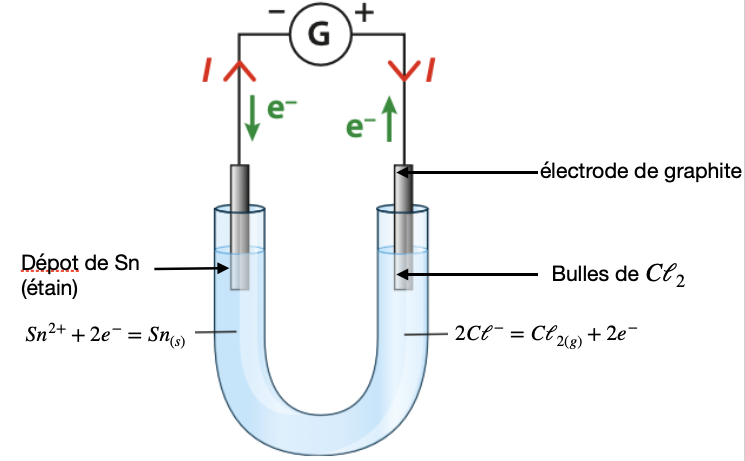
\includegraphics[width=10 cm]{figures/electrolyse_3}

Vidéo de l'expérience: \url{https://www.youtube.com/watch?v=0KI65y_b5y4}

\subsection{Obtention des équations redox}

On sait que :
\begin{itemize}
	\item Le courant I et le sens des $e^-$ est imposé par le générateur. 
	\item Initialement les seules espèces chimiques présentes sont: $C\ell^-$ et $Sn^{2+}$.
	\item Les couples sont $C\ell_{2(g)} / C\ell^-$ et $Sn^{2+} / Sn$.
	\item Equations redox des couples $$\trou{C\ell_{2(g)}} + 2e^- = \trou{C\ell^-}$$ $$Sn^{2+}+\trou{2e^-}=\trou{Sn}$$
\end{itemize}
 On en déduit que: 
\begin{itemize}
	\item Les électrons arrivent à gauche. Ils sont consommés selon $$\trou{Sn^{2+}}+2e^- = \trou{Sn}$$
	\item Les électrons qui partent de l'électrode à droite sont produits par $$2C\ell^-=C\ell_{2(g)}+\trou{2e^-}$$
\end{itemize}

\subsection{Interprétation chimique}

Durant l'électrolyse, on observe la réaction d'équation $$\trou{2C\ell^-+Sn^{2+}}\longrightarrow \trou{C\ell_{2(g)}+Sn_{(s)}}$$ 

\blocgris{Questions}{
On donne les concentrations initiales: $[Sn^{2+}]_i = 0,5$ mol/L et $[C\ell^-]_i = 1$ mol/L. Les activités du dichlore et de l'étain solide seront prises égales à 1.
\begin{enumerate}
	\item Calculer la valeur du quotient réactionnel à l'instant initial: $Q_{ri}$ ? 
	\item Sachant que la constante d'équilibre associée à la réaction ci-dessus vaut: K = \num{e-51}. Quel est le sens spontané de la réaction chimique.
	\item Justifier qu'il s'agit ici d'une réaction forcée.
\end{enumerate}
}

\etiquette{A savoir aussi... }
Les éléments des deux premières colonnes du tableau périodique sont les éléments du bloc s. Ils ont tous un ou deux électrons sur leur couche externe. Ils sont donc susceptibles de les perdre, ce qui fait d'eux des \trou{réducteurs}

\etiquette{Récap du cours sur électrolyse} \url{https://www.youtube.com/watch?v=w3lg9HDBMKw}


\newpage
\section{Application : dépôt d'un métal sur une surface}
L'un des procédés utilisé pour protéger l'acier de la corrosion est de l'isoler de l'atmosphère en le recouvrant
d'un revêtement métallique. Des plaques d'acier sont ainsi recouvertes d'une fine couche de zinc, on dit
qu'elles sont « galvanisées ».
Pour cela, on procède à l'électrolyse d'une solution aqueuse de sulfate de zinc (II) ($Zn^{2+}_{(aq)} + SO4
^{2-}_{4(aq)}$).
Dans ce bain électrolytique, on plonge une plaque à recouvrir et on utilise une lame de zinc comme seconde
électrode

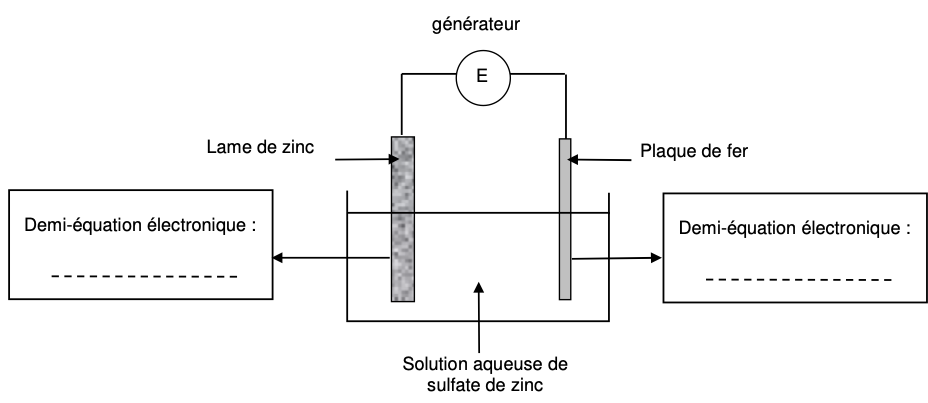
\includegraphics[width=12 cm]{figures/electrolyse_4.png}

\etiquette{Questions}
\begin{enumerate}
\item Compléter le schéma précédent en indiquant: où se forme le dépôt de zinc, la demi équation électronique traduisant la transformation ayant lieu sur la plaque de fer ($Fe^{2+}/Fe$);
\begin{itemize}
\item le sens de déplacement des électrons dans les conducteurs métalliques ;
\item les polarités du générateur ;
\item la demi équation électronique traduisant la transformation ayant lieu sur la lame de zinc.
\end{itemize}
La plaque d'acier a une surface totale de \SI{10}{m^2}. On veut déposer une couche de zinc de 0,10 mm
d'épaisseur, ce qui correspond à un volume de zinc égal à 1000 cm3. L'intensité du courant est maintenue
constante et égale à 1,0 kA.
\item  Calculer la masse de zinc à déposer.
\item En déduire la quantité d'électrons en mol devant traverser le circuit.
\item En déduire la durée de l'électrolyse.
\end{enumerate}
Données
\begin{itemize}
\item Masse volumique du zinc:$\rho=7,14g.cm^{-3}$
\item Masse molaire du zinc: M =65,4g/mol
\item Constante d'Avogadro: $ N_{A}=6,02\times10^{23}mol^{-1}$
\item Charge élémentaire: $e=1,60\times10^{-19}\:C$ 
\item Faraday: F=$96500\:C.mol^{-1}$
\end{itemize}
%\blocgris{Demi-équations}{
%Pour chacun des couples ci-dessous, écrire la demi-équation d'oxydo-réduction : 
%\begin{itemize}
%\item L'eau de javel est une solution d'ion hypochlorite $ClO^-$ oxydant du couple : $ClO^-/Cl^-$\\
%\trou{$ClO^-+H_20+2e-=Cl^-+2HO^-$}
%\item le dioxygène $O_2$ est l'oxydant du couple $O_2/H_2O$\\
%\trou{$O_2+4e-+4H^+=2H_2O$}
%\item le dichlore $Cl_2$ est l'oxydant du couple $Cl_2/Cl^-$\\
%\trou{$Cl_2+2e-=2Cl^-$}
%\item l'acide ascorbique ou vitamine C est le réducteur du couple $C_6H_6O_6/C_6H_8O_6$\\
%\trou{$C_6H_6O_6 +2H^+  = C_6H_8O_6$}
%\item le dihydrogène $H_2$ est le réducteur du couple $H^+/H_2$.\\
%\trou{$2H^+ +2e-=H_2$}
%\end{itemize}
%}

\etiquette{Exercices sur l'électrolyse}
\begin{itemize}
\item 1, 2, 8, 12 et 18 p 184
\item type bac: \url{https://www.labolycee.org/corrosion-et-protection-des-metaux}
\end{itemize}